\subsubsection{CRISP-DM}
\subsubsubsection{Definição}
CRISP-DM, ou\textit{ Cross-industry standard process for data mining}, é uma técnica aplicada no processo de mineração de dados, com uma série de tarefas a serem realizadas para chegar ao melhor resultado.
Segundo \citeAuthorPageYear{dmfd}, a mineração de dados não é algo feito uma vez e depois esquecido, o trabalho pode ser aplicado em outros projetos, servir de referência.
O ciclo de vida da mineração de dados contém seis fases, como apresentado na figura \ref{crispcycle}: entendimento do negócio, entendimento dos dados, preparação dos dados, modelagem, avaliação e implementação. 
A mineração de dados não termina uma vez que a solução é implementada.
\begin{figure}[H]
\centering
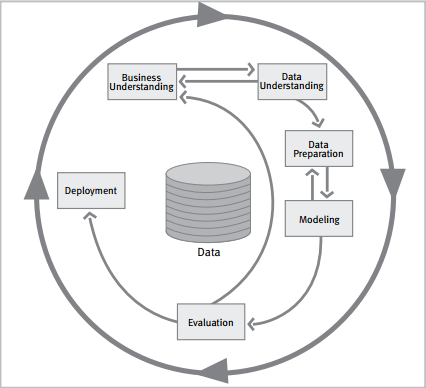
\includegraphics[height=6.2cm]{imagens/lifecycle.png}
\caption{Ciclo de vida (\citeauthor{crispmanual} \citeyear{crispmanual})}
\label{crispcycle}
\end{figure}
As fases tem diversas tarefas que são realizadas para completa-las e toda tarefa tem suas saídas. \citeAuthorPageYear{advancedDM} afirmam que esse processo não é rigio e precisa ser seguido ao pé da letra, além de que nem todos os processos precisam ser utilizados, caso a pessoa já tenha alguma experiência.
\subsubsubsection{Entendimento do negócio}
A primeira etapa do CRISP-DM é o entendimento do negócio, que foca em esclarecer os objetivos do negócio e seus requerimentos de uma perspectiva de negócio.

O primeiro objetivo da análise de dados é entender, sob uma perspectiva de negócio, o que o cliente deseja realizar. Segundo \citeAuthorPageYear{dmfd}, deve-se ter um entendimento claro do problema que se deseja abordar, o objetivo do negócio, as limitações e o impacto. Esse processo produz uma informação da situação do negócio, objetivo do cliente e o critério de sucesso.

Em seguida é realizada uma avaliação da situação. Segundo \citeAuthorPageYear{crispmanual}, essa tarefa consiste em um detalhamento maior dos recursos, limitações, premissas e outros fatores que devem ser considerados ao determinar os objetivos da análise de dados e do plano de projeto.

Outra etapa é determinar os objetivos da mineração de dados, por exemplo, como "prever quantas pessoas irão visitar uma loja no verão, de acordo com informações dos últimos 2 anos dessa loja".

E então produzir plano de projeto, ou seja, de acordo com \citeAuthorPageYear{crispmanual}, o plano desejado para atingir os objetivos da mineração de dados e desse modo, os objetivos do negócio. Esse processo produz o plano de projeto e avaliações iniciais de ferramentas e técnicas.

\subsubsubsection{Entendimento dos dados}
De acordo com \citeAuthorPageYear{dmfd}, na segunda etapa do projeto de mineração de dados, os dados têm que ser obtidos e deve-se verificar se eles são apropriados para as necessidades.

A primeira tarefa desse processo é coletar dados iniciais e então realizar, caso necessário, o carregamento dos dados em alguma ferramenta. Nessa tarefa é produzida uma lista de todos os \textit{datasets} adquiridos, junto com localizações, métodos realizados para coleta e problemas encontrados.

A próxima tarefa é descrever os dados, explora-se eles usando técnicas de visualização. Essa análise esta diretamente ligada aos objetivos da mineração de dados , de acordo com\citeAuthorPageYear{crispmanual}. Essa tarefa produz um relatório da exploração de dados, contendo descobertas iniciais ou hipóteses, e o seu impacto no restante do projeto.

Depois, é necessário verificar a qualidade dos dados, respondendo perguntas como "os dados estão completos?", "existem valores faltantes?". É criado um relatório da qualidade dos dados, com uma lista de problemas encontrados e suas soluções.

\subsubsubsection{Preparação dos Dados}
A maior parte do tempo gasto no processo de mineração de dados é na preparação deles, já que diversos tratamentos precisam ser feitos nos dados e isso nem sempre é tão simples. De acordo com \citeAuthorPageYear{dmfd}, a maior parte dos dados usados para mineração foi originalmente coletada e preservada para outros objetivos e precisa ser refinada antes de ser ficar pronta para a modelagem.

Essa parte tem duas saídas, antes das tarefas, que são: \textit{datasets}, dados produzidos e que serão usados para modelagem e \textbf{descrição do \textit{dataset}}.

A primeira tarefa é \textbf{selecionar os dados} que serão usados na modelagem, baseando-se nos objetivos da mineração de dados, qualidade e limites técnicos, segundo \citeAuthorPageYear{crispmanual}. É criada uma lista de dados que foram incluídos e excluídos e a razão para isso.

Segundo \citeAuthorPageYear{crispmanual}, Posteriormente é feita uma \textbf{limpeza dos dados}, que eleva a qualidade dos dados para o nível requerido pelas técnicas de análise selecionadas. De acordo com \citeAuthorPageYear{dmfd}, dificilmente os dados selecionados estarão perfeitamente limpos, mudanças precisarão ser feitas nos dados para atingir o nível necessário. Transformações nos dados são feitas para limpeza e possível impacto na análise de resultados. Nessa etapa é criado um relatório de limpeza de dados: que descreve as ações tomadas para lidar com os problemas encontrados anteriormente.

A tarefa seguinte é \textbf{Construir dados}, que consiste na criação de novos campos, dados agregados, ou novos formatos de dados. É produzida uma lista de atributos derivados a partir dos que já existem e explica como e por que eles foram gerados e uma lista de registros criados, junto com o motivo e como eles foram formados.

A próxima tarefa é \textbf{integrar dados}, já que existe a possibilidade deles estarem em diferentes \textit{datasets} e é necessário a integração desses dados para a próxima etapa, modelagem. A saída desse passo é: \textbf{dados fundidos}: fundir tabelas se refere a juntar duas ou mais tabelas que têm diferentes informações sobre o mesmo objeto. 

Por último, a tarefa \textbf{formatar dados} é aplicada. Dados frequentemente vêm em formatos que não são os convencionais para modelagem, segundo \citeAuthorPageYear{dmfd}, então conversões precisam ser feitas. O processo de preparação de dados deve ser finalizada com um \textit{dataset} pronto para modelagem e um relatório descrevendo o \textit{dataset}.

A saída é dados reformatados, convertidos para alguma unidade de medida única para todos os dados (como quilos, em peso).

\subsubsubsection{Modelagem}
É a etapa na qual alguma técnica de aprendizado de máquina é aplicada, testada e avaliada para encontrar padrões nos dados, como \textit{K-nearest neighbors}, \textit{Decision Tree }e etc. Dependendo do tipo de dados, diversos modelos podem ser aplicados, de acordo com \citeAuthorPageYear{advancedDM}.

O primeiro passo da modelagem é \textbf{selecionar a técnica de modelagem} que será usada. De acordo com \citeAuthorPageYear{crispmanual}, caso múltiplas técnicas sejam aplicadas, é preciso executar essa tarefa para cada uma delas. Nem todas as técnicas de modelagem serão úteis para as necessidades do negócio.

A escolha da técnica de modelagem depende muito dos tipos de dados, as técnicas, de acordo com \citeAuthorPageYear{advancedDM}, podem ser de associação, clusterização, previsão, etc.

De acordo com \citeAuthorPageYear{advancedDM}, em associação, a relação entre um item em uma transação de dados com outros itens, nessa mesma transação, é usada para prever padrões.

Na clusterização, segundo \citeAuthorPageYear{advancedDM}, dados não agrupados são agrupados utilizando técnicas automatizadas. Já a previsão é relacionado a técnicas de regressão. A ideia é descobrir a relação entre variáveis dependentes e independentes. Utilizando dados históricos, as técnicas de regressão, sejam lineares ou não, podem gerar uma curva de regressão que pode ser usada para realizar previsão.

Em seguida, o \textbf{teste de design} é gerado, ou seja, procedimentos ou mecanismos para testar a qualidade e validade do modelo, segundo  \citeAuthorPageYear{crispmanual}. Os dados geralmente são separados em dois conjuntos, o de treinamento e o de teste. O de treinamento é usado para construir o modelo e o de teste para validar ele. Nessa etapa é gerado descrito como planeja, treina, testa e avalia o modelo.

Depois, \citeAuthorPageYear{crispmanual} afirmam que é o momento de \textbf{construir o modelo}, rodar a ferramenta de modelagem para criar um ou mais modelos. Esse processo produz um documento com as configurações de parâmetros usados, modelos produzidos pela ferramenta e uma descrição deles.

Por fim, é a fase de \textbf{avaliar o modelo}, que sumariza os dados e ranqueia os modelos e também revisa as configurações dos parâmetros aplicados para tentar reajustá-los até encontrar a melhor possível.

\subsubsubsection{Avaliação}
Avaliar todo o processo: não só os modelos, mas também o processo empregado para a sua criação.

A primeira tarefa é \textbf{avaliar resultados}. Ela avalia o grau em que o modelo se adequa ao objetivo original do negócio e busca determinar se existe alguma razão para o modelo estar deficiente.

Ela também avalia o resultado da mineração de dados a respeito do critério de sucesso do negócio, \citeAuthorPageYear{dmfd} mostra que esse processo serve para dizer se o projeto atingiu ou não os objetivos definidos no início e seleciona os modelos que atingiram o critério selecionado.

Após a última tarefa, é feita uma \textbf{revisão do processo}, nesse ponto, os modelos resultantes aparentam ser satisfatórios para a necessidade do negócio, segundo \citep{crispmanual}. Essa é um passo usado para rever o processo, como algum problema que foi negligenciado. \citeAuthorPageYear{crispmanual} mostram que se deve sumarizar a revisão e ressaltar as atividades que não foram realizadas e aquelas que devem ser repetidas.

De acordo com \citeAuthorPageYear{dmfd}, a última fase é \textbf{determinar próximos passos}. A fase de avaliação é concluída com as recomendações para o próximo passo. Decidir se deve finalizar o projeto ou continuar o desenvolvimento. Para \citeAuthorPageYear{crispmanual}, essa fase também inclui a análise das despesas e recursos restantes, que tem influencia na decisão.
Essa etapa produz uma lista de possíveis ações e a decisão.

\subsubsubsection{Implementação}
O objetivo dessa última parte é a implementação do modelo.
O primeiro passo, de acordo com \citeAuthorPageYear{crispmanual} é o plano de implementação, usando os resultados da avaliação e determina a estratégia de implementação. 

A primeira parte é gerar um plano que sumariza as estratégias para implementação, os passos necessários e como realizar.
Posteriormente é feito um \textbf{Plano de monitoramento e manutenção}, conforme \citeAuthorPageYear{dmfd} diz, a mineração de dados é um ciclo, então existe a necessidade continuar envolvida com os modelos enquanto eles são integrados ao dia-a-dia. Para \citeAuthorPageYear{crispmanual}, a preparação cuidadosa das estratégias de manutenção ajuda a evitar longos períodos desnecessários de uso incorreto dos resultados da mineração.

Em seguida é produzido um plano de monitoramento e manutenção que sumariza todas as estratégias de manutenção e monitoramento, incluindo os passos necessários para realizá-los.
Em seguida, é feito um \textbf{Relatório Final}, um sumário do projeto e das experiências ou uma apresentação final e compreensível dos resultados da mineração.
Essa etapa produz o relatório final, que sumariza todo o projeto ao juntar todos os relatórios criados até o momento, de acordo com \citeAuthorPageYear{dmfd} e apresentação final, um encontro realizado na conclusão do projeto com seu cliente.

Por último, é feita uma \textbf{revisão do projeto} na qual o time se reúne e discute o que deu e não deu certo, o que pode e não pode ser feito novamente, e coisas que devem ser evitado.
A saída é uma documentação de experiência que sumariza a experiência ganha com o projeto, como erros e acertos, dicas de como selecionar os melhores modelos para situações semelhantes etc.
